\chapter*{The course} \label{chp:course}
\lecture{2024-08-02}{}

\href{https://sites.google.com/view/subhojoy/ma-231-2024}{Course website}

\section*{Timings} \label{sec:timings}
\textbf{Lectures:} MWF 3--4 pm\\
\textbf{Tutorial:} Tue 5--6 pm

\section*{Grading} \label{sec:grading}
\begin{itemize}
    \item Quizzes: 
    \item Midterm: 
    \item Final:   
\end{itemize}

\chapter{Introduction} \label{chp:intro}
Many objects in mathematics can be described as either \emph{numbers}
(arithmetic, algebra) or \emph{shapes} (geometry).

\emph{Topology} is geometry made ``flexible''.
How so? Topology allows for deformations, that retain a notion of
``proximity'' between points.

The following two triangles are identical for the topologist.
\begin{center}
    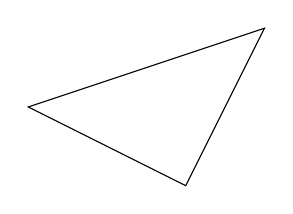
\begin{tikzpicture}
        \draw (0,0) -- (2,-1) -- (3,1) -- cycle;
    \end{tikzpicture}%
    \quad%
    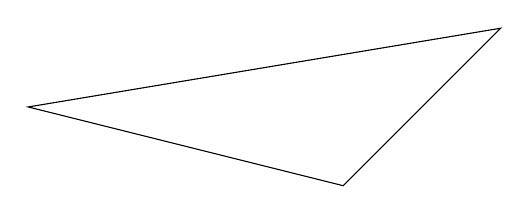
\begin{tikzpicture}[xscale=2]
        \draw (0,0) -- (2,-1) -- (3,1) -- cycle;
    \end{tikzpicture}
\end{center}
So are a sphere and an ellipsoid.
\begin{center}
    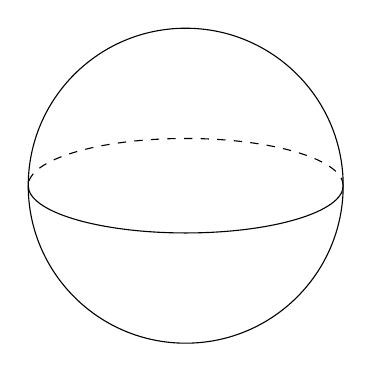
\begin{tikzpicture}
        \draw (0,0) circle (2);
        \draw (-2,0) arc (180:360:2 and 0.6);
        \draw[dashed] (2,0) arc (0:180:2 and 0.6);
    \end{tikzpicture}%
    \quad%
    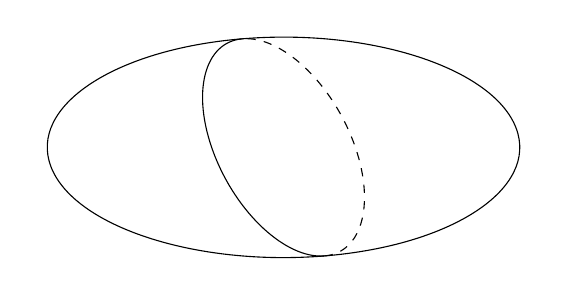
\begin{tikzpicture}[xscale=1.5, yscale=0.7, rotate=-80]
        \draw (0,0) circle (2);
        \draw (-2,0) arc (180:360:2 and 0.6);
        \draw[dashed] (2,0) arc (0:180:2 and 0.6);
    \end{tikzpicture}
\end{center}

Why is this useful?

Often, we only need to understand shapes qualitatively.
For example, a disk and a sphere look somewhat similar.
However, a qualitative difference is that the disk has a boundary,
while the sphere does not.
\begin{center}
    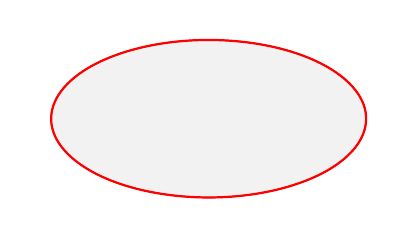
\begin{tikzpicture}[yscale=0.5, rotate=30]
        \draw[fill=gray!10] (0,0) circle (2);
        \draw[red, thick] (0,0) circle (2);
    \end{tikzpicture}%
    \quad%
    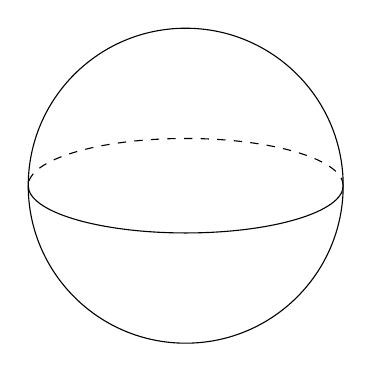
\begin{tikzpicture}
        \draw (0,0) circle (2);
        \draw (-2,0) arc (180:360:2 and 0.6);
        \draw[dashed] (2,0) arc (0:180:2 and 0.6);
    \end{tikzpicture}
\end{center}

\subsection*{Dynamical systems} \label{sec:dynamical}
Shapes arise while modelling physical systems.
A robotic arm may be described by some angles,
and so might the solar system.
Two friends playing hide-and-seek might be described by their positions.

Such parameters often lend themselves to a simple geometric description
in a \emph{phase space} or \emph{configuration space}.

Poincar\'e discussed the stability of the solar system around 1890
by studying the topology of the phase space.

\subsection*{Knot theory} \label{sec:knot}
Whether a knot can be untied without cutting is a topological question.
A qualitative understanding of the knot is sufficient.

\subsection*{Graphs} \label{sec:graphs}
% \begin{center}
%     \begin{tikzpicture}
%         \node[draw, circle] (a) at (0,0);
%     \end{tikzpicture}
% \end{center}

\section{What can you expect?} \label{sec:overview}
The course will cover point-set topology for more that half the semester.
Problems will bring out logical thinking, and sometimes your visual
imagination will be of great use.

Later, we will cover algebraic invariants, which form a bridge between
numbers and shapes.

\chapter{Set theory} \label{chp:set}
\begin{definition}[Maps] \label{def:maps}
    A \emph{map} or a \emph{function} between two sets $A$ and $B$
    assigns to every element of $A$ a unique element of $B$.
    \begin{align*}
        f\colon A &\to B \\
        a &\mapsto f(a)
    \end{align*}

    An \emph{injective} or \emph{one-to-one} map is one where distinct
    elements of $A$ are mapped to distinct elements of $B$. \[
        f(x) = f(y) \implies x = y
    \]

    A \emph{surjective} or \emph{onto} map is one where for every $b \in B$
    there exists an $a \in A$ that maps to $b$. \[
        f(A) = B
    \]

    A \emph{bijective} map is one that is both injective and surjective.
\end{definition}

\begin{proposition*}
    There is a bijection between $\R$ and $\R^2$.
\end{proposition*}
\begin{proof}
    We will use \cref{thm:schroder-bernstein}.
    $f = x \mapsto (x, 0)$ is an injective map from $\R$ to $\R^2$.
    For finding an injection, $g\colon \R^2 \to \R$, we will go via the
    map $\what{g}\colon (0, 1)^2 \to (0, 1)$.

    This is sufficient because $\arctan$ provides a nice bijection
    between $(0, 1)$ and $\R$ (and hence $(0, 1)^2$ and $\R^2$).

    Given $(x, y) \in (0, 1)^2$,
    let $0.x_1x_2x_3\dots$ and $0.y_1y_2y_3\dots$ be the binary
    expansions of $x$ and $y$ respectively.
    Interleave the bits to get $0.x_1y_1x_2y_2x_3y_3\dots$.
    (If we declare the expansions to be non-terminating, they are unique.)
    This is a bijection.
\end{proof}

\begin{theorem*}[Schr\"oder-Bernstein] \label{thm:schroder-bernstein}
    If $A$ and $B$ are sets such that there is an injective map
    $f\colon A \to B$ and a surjective map $g\colon A \to B$,
    then there is a bijection $h\colon A \leftrightarrow B$.
\end{theorem*}
\begin{proof}[Following McMullen's notes]
    WLOG assume $A$ and $B$ are disjoint.
    Let $F = f \cup g\colon A \cup B \to B \cup A$ be the union of the two
    maps (as sets).
    That is, \[
        F(x) = \begin{cases}
            f(x) & \text{if } x \in A, \\
            g(x) & \text{if } x \in B.
        \end{cases}
    \] For any $x$, we say that $x$ is the \emph{parent} of $F(x)$,
    which is the \emph{child}.

    Now note the following.
    \begin{enumerate}
        \item Each element of $A \cup B$ is a parent and has a single child.
        \item There may be elements in $A \cup B$ that are not children.
            Call them \emph{godfathers}.
        \item Each child has a unique parent.
    \end{enumerate}
    Consider any element $x \in A \cup B$.
    We have two possibilities.
    \begin{enumerate}
        \item $\dots \mapsto x'' \mapsto x' \mapsto x$.
        \item $y \mapsto \dots \mapsto x' \mapsto x$,
            where $y$ is a godfather.
    \end{enumerate}
    We divide $A$ into three mutually disjoint sets, $A_0$, $A_A$ and $A_B$.
    \begin{align*}
        A_0  &= \set{x \in A
                    \mid \text{possibility (i) happens}}, \\
        A_A &= \set{x \in A
                    \mid \text{possibility (ii) happens and $y \in A$}}, \\
        A_B &= \set{x \in A
                    \mid \text{possibility (ii) happens and $y \in B$}}.
    \end{align*}
    Similarly, define $B_0$, $B_A$ and $B_B$.

    Now $F\vert_{A_0} : A_0 \to B_0$ is a bijection,
    $F\vert_{A_A} : A_A \to B_A$ is a bijection, and
    $F\vert_{B_B} : B_B \to A_B$ is a bijection.
    Flipping the last bijection gives a bijection
    $F\vert_{B_B}^{-1} : A_B \to B_B$.

    Now we can define a bijection $h\colon A \to B$ as
    $h = F\vert_{A_0} \cup F\vert_{A_A} \cup F\vert_{B_B}^{-1}$.
\end{proof}
